%\author{D. Crews}

\documentclass[12pt]{article}

\usepackage{amsmath}
\usepackage{graphicx}
\usepackage{bm}
\usepackage{mathabx}
\usepackage[margin=1.0in]{geometry}
\usepackage[english]{babel}
\usepackage{enumitem}
\usepackage{hyperref}
%\usepackage{roman}

\begin{document}
\title{\Large {\bf AA 321 | Aerospace Laboratory\\Lab One: q-Calibration of the 3x3 Wind Tunnel}\\[1ex]
  University of Washington}
\date{\today}
\maketitle
%\tableofcontents

\section{Objectives}\label{objs}
The purpose of this experiment is to introduce you to simple flow field characteristics in a wind tunnel (in this case the department’s 3x3-ft Wind Tunnel) by analyzing basic measurements of dynamic pressure ($q$). This experiment consists of two parts:
\begin{enumerate}
\item Calibration of dynamic pressure along the wind tunnel’s vertical axis, i.e., the Z-axis,
\item Consideration of the uniformity of q along said Z-axis.
\end{enumerate}

\section{Background}
The 3x3 wind tunnel is housed in one of the first buildings associated with aeronautical engineering at UW, built in 1917 on a grant from William Boeing. The current wind tunnel model is an open-return design, meaning that air is exhausted through a diffuser and returns around the sides of the tunnel to the inlet section (see Fig. \ref{tunnel}). 

\begin{figure}[h]
  \centering
  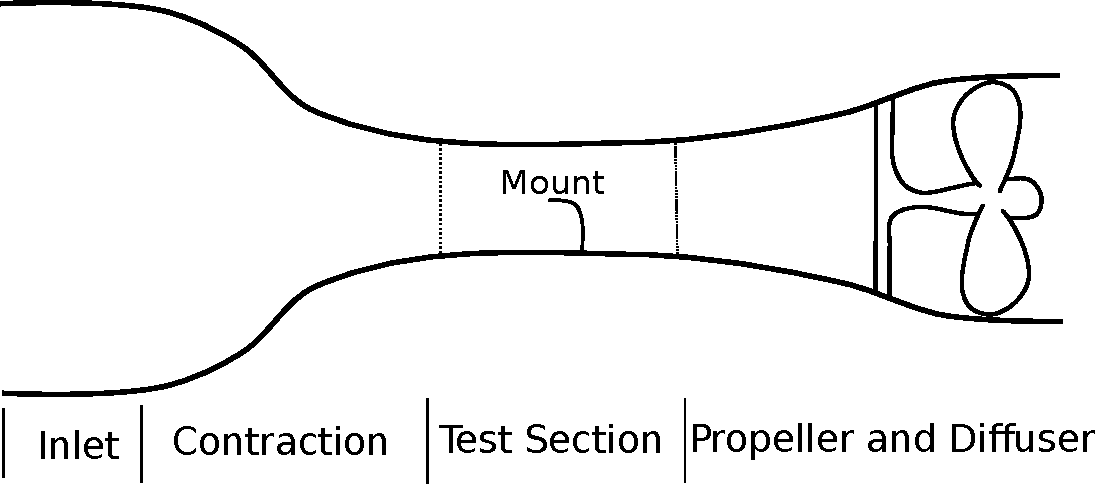
\includegraphics[width=0.5\textwidth]{tunnel}\\
  \caption{Simple schematic of open-return wind tunnel featuring inlet, contraction, test section, and propeller driven by 200-hp motor.}\label{tunnel}
\end{figure}

One of the simplest methods for infering flow speed uses the energy conservation relation
\begin{equation}
  p + q = p_{\text{t}}
\end{equation}
where $p$ is static pressure (the internal or microscopic energy density), $q = \frac{1}{2}\rho v^2$ is dynamic pressure (the bulk or macroscopic energy density), and $p_t$ is total pressure. Total pressure (or total energy density in a given frame of reference) is a constant of motion and is measured by stagnating the flow (i.e. bringing it to a halt), so that dynamic pressure $q$ is locally zero and the static pressure $p$ becomes the total pressure. For this reason total pressure is also known as the stagnation pressure. Comparison of total and static pressures determines the dynamic pressure as $q = p_t - p$. The pitot-static tube, shown in Fig. \ref{pitot}, operates by exposing pressure transducers to i) flow halted through an upwind-facing orifice, and ii) flow unobstructed through ports orthogonal to flow \cite{liepmann}.

\begin{figure}[h]
  \centering
  
\includegraphics[width=0.5\textwidth]{pitot_static}\\
  \caption{The pitot-static tube measures total pressure through port $A$ and static pressure through ports $B$, each of which are connected to pressure transducers at C.}\label{pitot}
\end{figure}

To complete the measurement of velocity, the fluid density $\rho$ must be determined. The density $\rho$ is a function of the state of the gas (almost always via the ideal gas relation, and in this case rather weakly due to changes in air temperature during the experiment). As one can imagine, the pitot tube is not a perfect measuring device and there are a few sources of error. Can you think of what they may be?

An ideal flow through the test section of the tunnel would be of vertically uniform velocity. However, fluid viscosity imposes the \textit{no-slip boundary condition} where velocity $v$ is zero on static surfaces. The transition region where flow velocity varies from static ($v=0$) to unobstructed ($v=v_{\text{free}}$) is known as a boundary layer. Figure \ref{boundary} shows a typical laminar boundary layer velocity profile. The \textit{boundary layer thickness} $\delta$ is defined as the width from the wall to where the flow obtains $99\%$ of its free speed.

\begin{figure}[h]
  \centering
  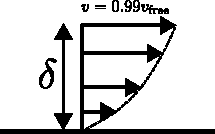
\includegraphics[width=0.5\textwidth]{boundary_layer}\\
  \caption{Velocity profile of a laminar boundary layer. The thickness $\delta$ is a measure of the width of depressed velocity and is defined from the wall up to $99\%$ of the free velocity.}\label{boundary}
\end{figure}

\subsection{Collected data}
In this experiment, data was collected in three experiments:
\begin{itemize}
\item A sweep of dynamic pressures (at nominal $q=10, 20, 30, 40,$ and $50$ psf) at three vertical ($z$) positions,
\item Measurements of flow speed at the top boundary for various dynamic pressures,
\item A full $z$-sweep of the tunnel at maximum nominal $q$ ($\sim 50$ psf).
\end{itemize}
Data was collected and saved to comma-separated value (csv) files. The relevant columns are the third, fourth, and fifth. The third column indicates the $z$ coordinate in inches, where $z=0$ is the top of the test section. The fourth column lists the indicated-$q$ (in psf) of the tunnel, which is a \textit{rough estimate} of wind speed inferred from pressure ports in the inlet and contraction sections. The fifth column lists the dynamic pressure (in psf) as measured by the pitot static tube. Note that there is considerable uncertainty in all measurements. For example, at a nominal $z=0$ the flow velocity is not going to be exactly $v=0$. This is because the pitot tube is actually measuring a half tube-diameter away the wall, and the stagnation pressure measured is an average over the tube's inlet diameter.

\section{Analysis tasks}
Having received the testing team's data, consider the following questions during your team's analysis. You are under no obligation to answer these questions in any particular order; instead, consider them as a whole and in whichever order will make the most sense for presentation to your audience.

\begin{enumerate}
\item \textbf{q-Sweep at fixed $z$-positions}: The testing team has found that the calibration equation for the pitot-static probe is $q_{\text{true}} = 1.012 q_{\text{probe}}$. Plot the difference $\Delta q \equiv q_{\text{true}} - q_{\text{ind}}$ for the three $z$-positions investigated in the first batch of collected data. Include error bars.
  \begin{itemize}
  \item \textbf{Data reduction}: To obtain a measurement from the raw data, visualize the indicated and probe $q$'s for a given $z$-location. Identify a collection of data points corresponding to a certain nominal wind speed. Obtain a measurement and its error bars by calculating the mean and variance of the identified raw data points.
  \item \textbf{Consider}: How do these values of $q$ compare? Explain discrepancies between $q_{\text{ind}}$ and $q_{\text{true}}$. If there are discrepancies at different $z$-locations, explain why.
  \item \textbf{Functional relation}: Calculate and plot the true airspeed of the wind tunnel (in ft/sec, mph, and m/s) as a function of $q_{\text{ind}}$.
  \item \textbf{Power requirements}: Assuming a fan efficiency of $\eta = 0.85$, calculate the power (in both hp and kW) required to drive the wind tunnel at $q_{\text{ind}} = 40$ psf. (hint: the test section has a square cross-section of 3 ft x 3 ft.
  \end{itemize}
\item \textbf{Boundary layer}: Data was collected near the boundary for various $z$-positions at $q=10, 20, 30, 40$ and $50$ psf. Plot the velocity profile $v$ against position $z$ for the various speeds. Estimate the boundary layer thickness $\delta$ in each case.
\item \textbf{Full $z$-sweep at fixed $q$}: The data collected at $q_{\text{ind}} = 50$ psf extended beyond the boundary layer and close to the bottom of the tunnel. The pitot tube then had to be manually adjusted to be flush against the bottom of the tunnel and then swept up out of the bottom boundary layer.
  \begin{itemize}
  \item \textbf{Consider}: By consideration of both data sets, plot $q_{\text{true}}$ vs. $z$ in the test section.
  \item \textbf{Fluctuations}: Obtain (to the best of your team's ability) error bars as well. Comment on i) the variations observed in $z$ in comparison to ii) the magnitude of the estimated error bars.
  \item \textbf{Flow quality}: What could be done to improve flow quality in this test section?
  \item \textbf{Temperature}: Temperature varied from $\sim 18^\circ$ C to $\sim 22^\circ$ C during data collection. Why does this matter and what is its effect (qualitatively) on analysis?
  \end{itemize}
\end{enumerate}

\bibliographystyle{plain}
\bibliography{lab1}

\end{document}